\documentclass{beamer}

% Theme and page layout
\usetheme{gapz}
\setbeamertemplate{navigation symbols}{}

% Fonts
\usepackage{fontspec}
\defaultfontfeatures{Mapping=tex-text,Scale=MatchLowercase,Numbers=Lining}
%\setsansfont[
%	ItalicFont = Whitney MediumItalic,
%	BoldFont = Whitney Semibold,
%	BoldItalicFont = Whitney SemiboldItalic,
%	SmallCapsFont = Whitney MediumSC
%]{Whitney Medium}

% Language
\usepackage{polyglossia}
\setdefaultlanguage{english}

% Graphics
\usepackage{graphicx}
\graphicspath{{./images/}}
\usepackage{multicol}

\title{Three-dimensional modeling and printing project}
\subtitle{Third-year project}
\author[V. Duvert, A. Lubineau, C. Naud, J. Packer, F. Ribon]{\scriptsize
Vincent~Duvert \\ Antoine~Lubineau \\ Caroline~Naud \\ James~Packer \\ Florian~Ribon}
\date{from January 23 to March 16, 2012}

\titlegraphic{
\includegraphics[width=4cm]{inp-enseeiht}}

\begin{document}

\frame{\titlepage}

\section{Presentation of the project}

\subsection{Clients}
\begin{frame}
	\frametitle{}
	
	\begin{block}{The VORTEX team of IRIT}
		\begin{itemize}
		\item IRIT: a research institute in computer science from Toulouse, mostly working on graphic computing,
		\item VORTEX: Visual Objects: from Reality To EXpression,
		\item Recently acquired an uncalibrated Ultimaker 3D printer.
		\end{itemize}
    \end{block}
    
    \begin{center}
		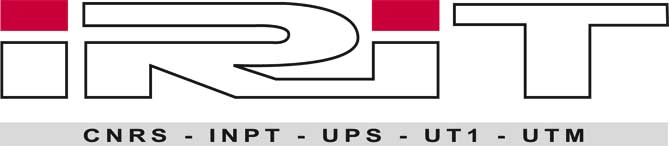
\includegraphics[width=5cm]{irit}
	\end{center}
    
\end{frame}

\subsection{Objectives}
\begin{frame}
	\frametitle{The main client's requests}
	\begin{block}{Main goals of the project} 
	\begin{itemize}
		\item Open-source modeler able to import, model, deform and \textbf{correct} virtual 3D objects,
		\item Interactions using the touchscreen,
		\item Export meshes to the printer,
		\item Print as realistically as possible,
	\end{itemize}
    \end{block}
    
    \begin{block}{The final users}
    	\begin{itemize}
		\item The VORTEX team,
		\item Some artists from Artilect that we visited or artists students.
		\end{itemize}
    \end{block}

\end{frame}

\subsection{Resources}
\begin{frame}
	\frametitle{}
	
	\begin{block}{The project team}
		\begin{itemize}
		\item Five final year students at ENSEEIHT, Computing and Applied Mathematics department
		\item Several followed the “multimedia” option in third year
		\item Project manager: Caroline Naud
		\end{itemize}
    \end{block}
    
    \begin{block}{The material resources}
    	\begin{itemize}
    	\item Ultimaker 3D printer with a roll of PLA plastic in room F117 at ENSEEIHT,
    	\item Computer with dual-touch screen Acer T231H.
		\end{itemize}
    \end{block}
      
\end{frame}

\begin{frame}
	\frametitle{Ultimaker 3D printer}
	
	\begin{columns}[t]
  	\begin{column}{5cm}
  		\begin{figure}
		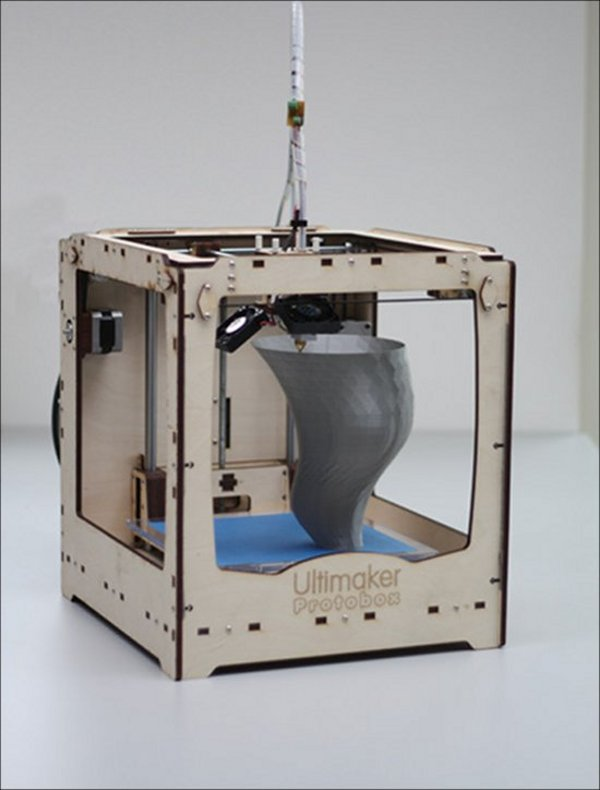
\includegraphics[width=4cm]{Ultimaker}	
		\end{figure}
  	\end{column}
  
  	\begin{column}{5cm}
  		\begin{block}{Process description}
  		\begin{enumerate}
  		\item The mesh is sliced into layers,
  		\item The associated instructions are generated,
  		\item The corresponding Gcode is sent to the printer,
  		\item The object is created by laying down successive layers of material.
  		\end{enumerate}
 	 	\end{block}   
  	\end{column}
 	\end{columns}  
\end{frame}



\section{Architecture of the project}

\begin{frame}
	\frametitle{A four steps application}
	
	\begin{block}{}
		\begin{itemize}
			\item Modeler: to import/create STL and PLY meshes and to pre-process them,
			\item G-code generator: to generate printing instructions,
			\item Printer's driver: to send the instructions including special parameters such as the temperature of the nozzle,
			\item Printer: to create the final object.
		\end{itemize}
	\end{block}
	
\end{frame}


\begin{frame}
	\frametitle{From the modeler to the printer…}

    \begin{center}
		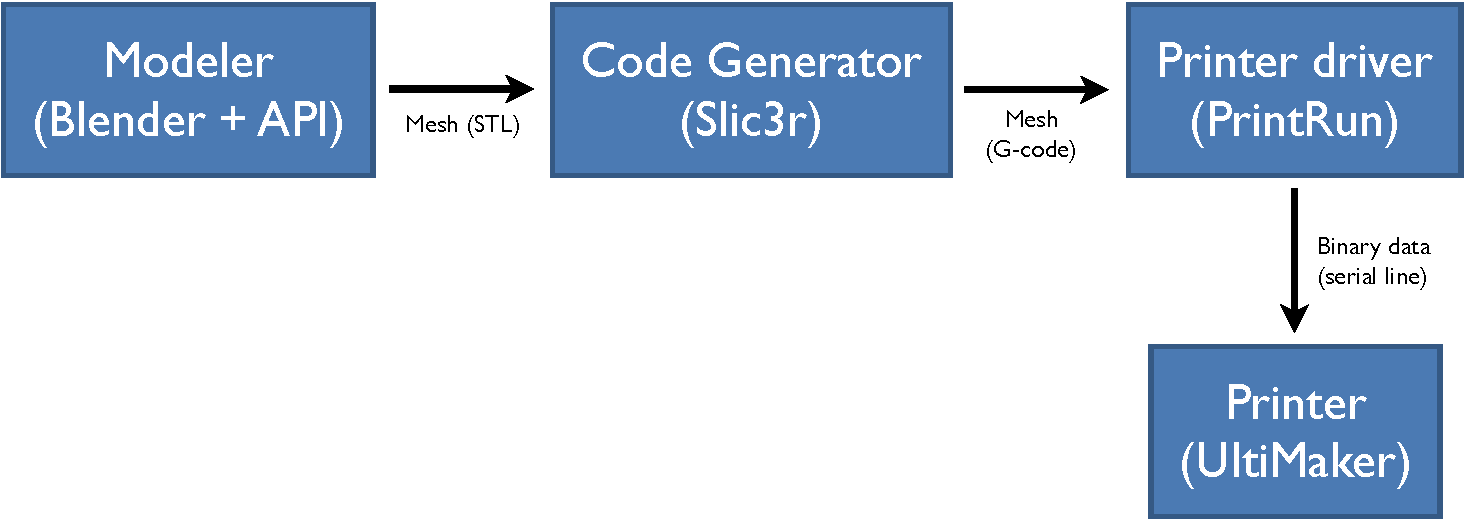
\includegraphics[width=10cm]{schema}	
	\end{center}
	
\end{frame}

\section{Project management}

\begin{frame}
	\frametitle{}
	\begin{block}{The tools}
    \begin{itemize}
		\item A web-based project management system: Chiliproject (Gantt charts, calendars, documents, wiki, notifications\ldots ),
		\item Code management with Git.
	\end{itemize}
	\end{block}
	
	\begin{block}{The external help}
    \begin{itemize}
		\item Our industrial supervisor from Airbus: Lionel Cremel,
		\item The weekly meetings with the supervisor, 
		\item The current weetings with the clients.
	\end{itemize}
	\end{block}
\end{frame}

\begin{frame}
	\frametitle{The V cycle management strategy}
	\begin{center}
		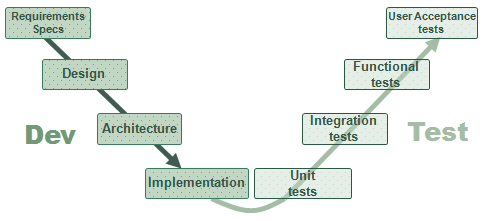
\includegraphics[width=10cm]{VCycle}	
	\end{center}
    
\end{frame}

\begin{frame}
	\frametitle{The macroscopic planning}

    \begin{center}
		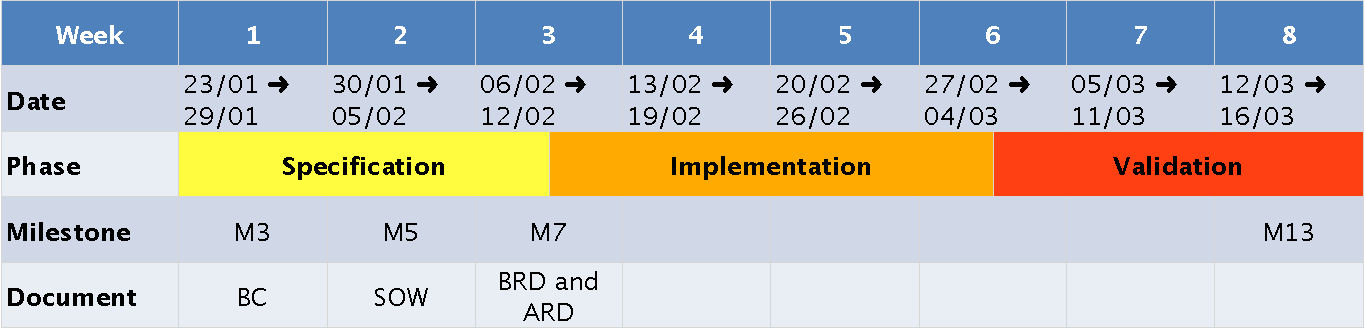
\includegraphics[width=\textwidth]{planning}	
	\end{center}
	
		Airbus milestones to respect: mainly documents to provide.
	
\end{frame}



\section{The main specifications}

\subsection{About the global application}
\begin{frame}
	\frametitle{}
	 \begin{block}{The application characteristics}
		\begin{itemize}
			\item Must be fully open source,
			\item Must be usable on both Linux Ubuntu and Windows (if possible),
			\item Must be delivered as an archive.
		\end{itemize}
    \end{block}
\end{frame}
    
\subsection{About the modeler}
\begin{frame}
	\frametitle{}
	 \begin{block}{The modeler characteristics}
		\begin{itemize}
			\item STL and PLY meshes import and STL meshes export required.
		\end{itemize}
    \end{block}
    
    \begin{block}{The online interactions required on the meshes}
		\begin{itemize}
			\item Add, remove, translate a vertex,
			\item Smooth a surface (automatically add faces, etc.),
			\item Cut an object.
		\end{itemize}
			$\Longrightarrow$ week complexity required
    \end{block}
    
    \begin{block}{The offline interactions required on the meshes}
		\begin{itemize}
			\item Mesh defaults detected and corrected before printing.
		\end{itemize}
			$\Longrightarrow$ high complexity accepted
    \end{block}

\end{frame}

\subsection{About the documentation}
\begin{frame}
	\frametitle{}
	 \begin{block}{The required documentation}
		\begin{itemize}
			\item \textbf{User documentation:} to use the application properly just by reading it. It should include the limits of the application,
			\item \textbf{Technical documentation:} so that the client or an other team can continue the work if needed,
			\item \textbf{Installation paper:} to enable the user to get an operational application from the initial archive.
		\end{itemize}
    \end{block}    

\end{frame}

\section{Our technical solutions and results}

\subsection{Choice of the 3D processing software}
\begin{frame}
	\frametitle{By the all team}
		\small $\Longrightarrow$ Conception of a modeler from scratch excluded. \\
		\small $\Longrightarrow$ Choice reduced to two editors: Blender and Meshlab.
    \begin{columns}[t]
  	\begin{column}{5cm}
  		\begin{block}{Meshlab}
  		\small \textit{Advantages}:
  		\begin{itemize}
  		\item Very light application,
  		\item Preexisting functions for mesh correction.
  		\end{itemize}
  		
  		\small \textit{Drawbacks}:
  		\begin{itemize}
  		\item No integrated interaction.
  		\end{itemize}
 	 	\end{block}   
  	\end{column}
  
  	\begin{column}{6cm}
  		\begin{block}{Blender (final choice)}
  		\small \textit{Advantages}:
  		\begin{itemize}
  		\item Preexisting interactions,
  		\item Powerful Python API,
  		\item A lot of documentation.
  		\end{itemize}
  		
  		\small \textit{Drawbacks}:
  		\begin{itemize}
  		\item Useless things for printing purposes
  		\end{itemize}
 	 	\end{block}   
  	\end{column}
 	\end{columns}  
    
\end{frame}

\subsection{Mesh correction integration}

\begin{frame}
	\frametitle{In charge: Florian Ribon}
    \begin{block}{Characteristics needed for printing}
		\begin{itemize}
		    \item \textbf{Watertight}: there is no hole in the mesh,
            \item \textbf{Manifold}: each edge belongs to exactly 2 faces.
		\end{itemize}
    \end{block}

    \begin{block}{Our correction tools}
		\begin{itemize}
		    \item Possibility to \textit{check} if the mesh is correct,
			\item If not, two methods are available to \textit{repair} it.
		\end{itemize}
    \end{block}

\end{frame}

\begin{frame}
	\frametitle{In charge: Florian Ribon}

    \begin{columns}[t]
  	\begin{column}{5cm}
        \begin{block}{Different manifoldness corrections}
		    \begin{itemize}
			    \item Simple cleaning\\\small(non destructive),
			    \item Or total repairing\\\small(destructive).
			    \item Optionnaly: fast-processing.
		    \end{itemize}
        \end{block}
    \end{column}

    \begin{column}{6cm}
        \begin{center}
		    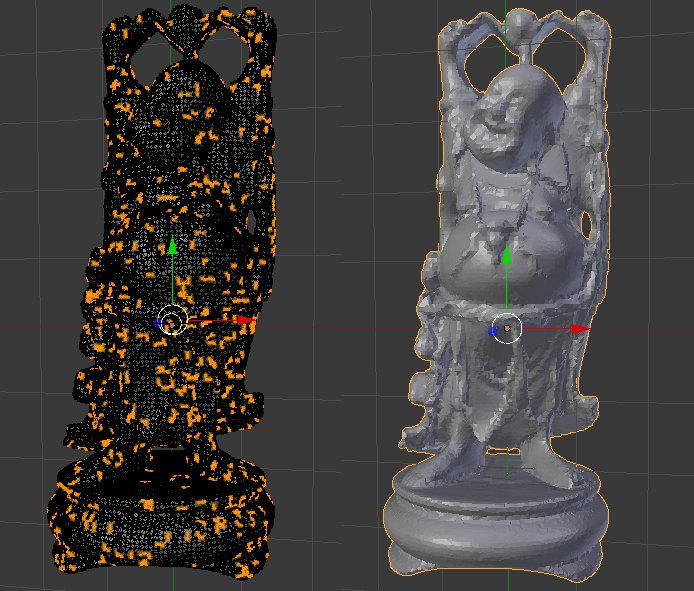
\includegraphics[height=.7\textheight]{repair}
	    \end{center}
    \end{column}

    \end{columns}
\end{frame}

\begin{frame}

    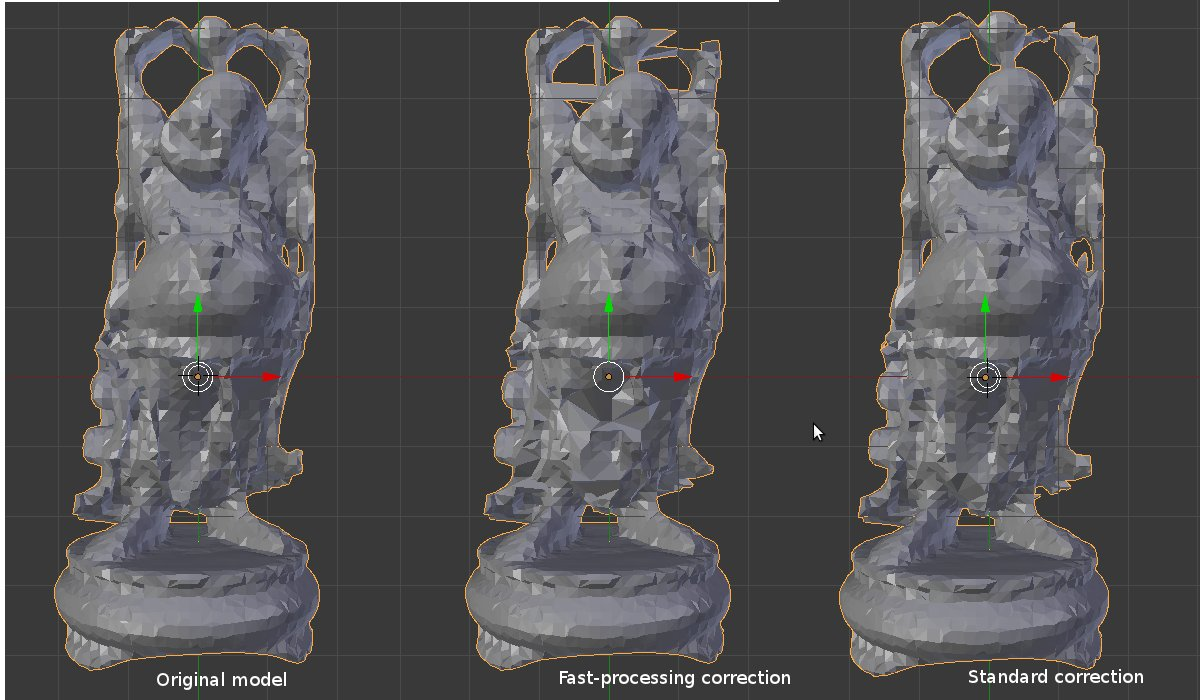
\includegraphics[width=1\textwidth]{damages}

\end{frame}

\begin{frame}
	\frametitle{In charge: Vincent Duvert and Antoine Lubineau} 
	\begin{block}{Difficult cases}
		\begin{itemize}
			\item No large planar faces? Create them by cutting the object (with the help of the user),
			\item Another option is to create a socle for the object.
		\end{itemize}
    \end{block}

	\begin{center}
		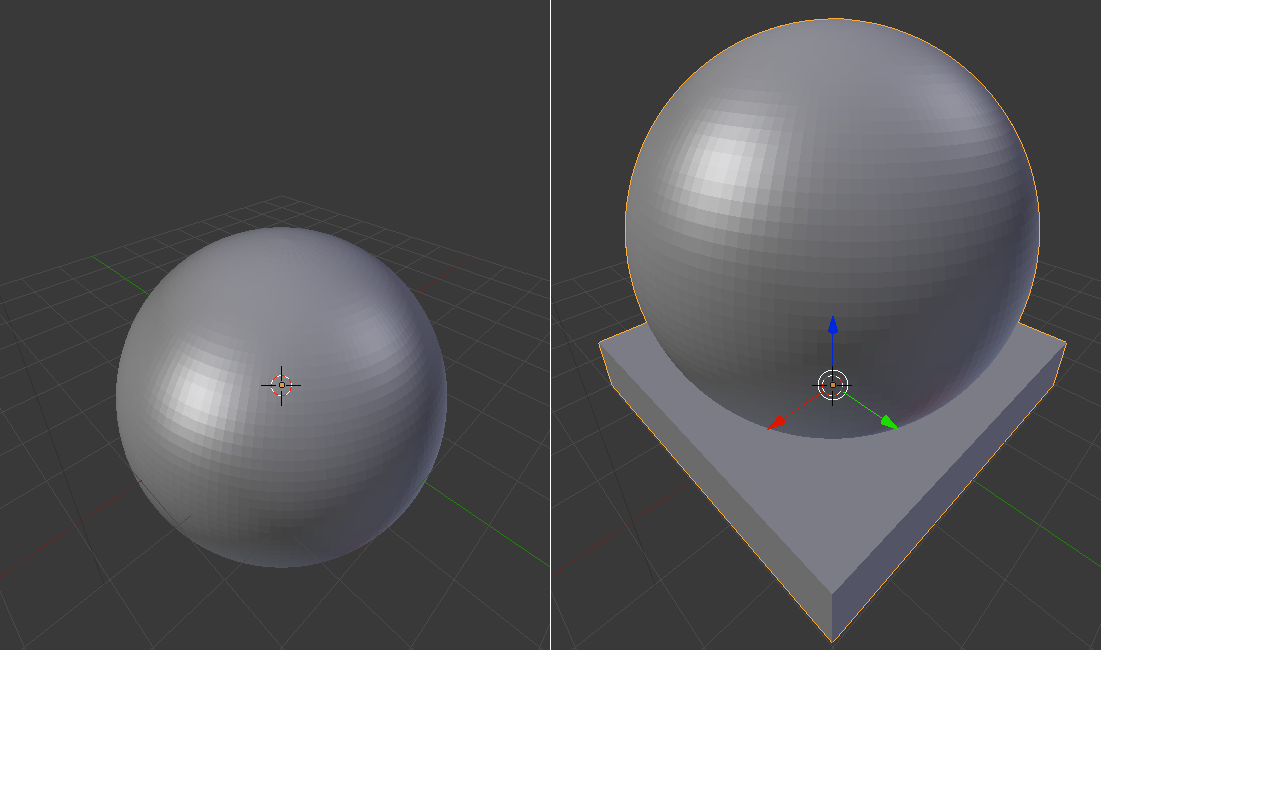
\includegraphics[width=.7\textwidth]{pf_socle}
	\end{center}
    
\end{frame}

\subsection{Modifications in Blender's GUI}
\begin{frame}
	\frametitle{In charge: Caroline Naud}

    \begin{block}{A new screen for Blender}
Possibility in Blender to manually modify the interface and to register it as the default one.
    \end{block}
    
    \begin{block}{A new panel}
    \begin{itemize}
	\item Addition of a new panel named “Mesh verification” thanks to the Blender Python API,
	\item Insertion of buttons appearing conditionally and calling the implemented mesh corrections.
	\end{itemize}
    \end{block}
\end{frame}

\begin{frame}
	\frametitle{In charge: Caroline Naud}
    \begin{center}
		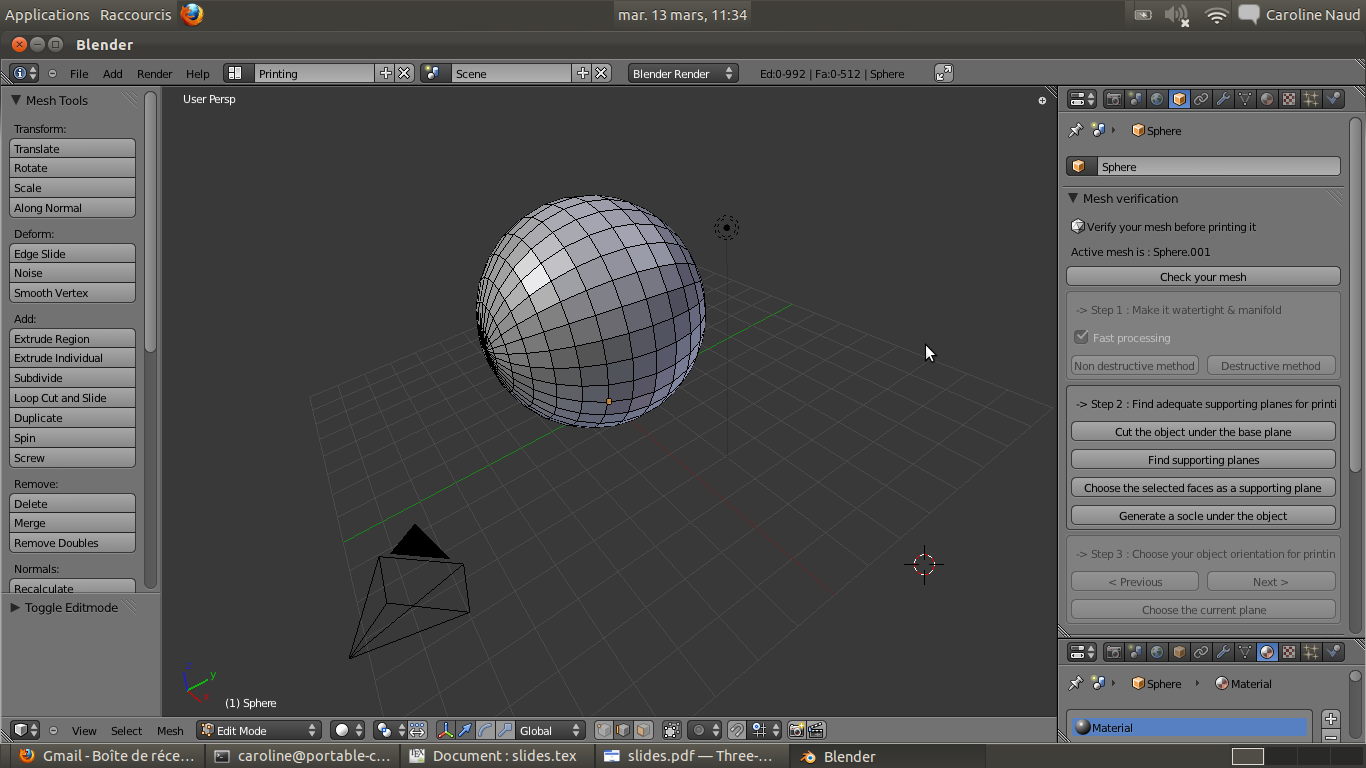
\includegraphics[height=.8\textheight]{Panel}
	\end{center}
\end{frame}

\begin{frame}
	\frametitle{In charge: Vincent Duvert}
    \begin{block}{Progress display}
	\begin{itemize}
	\item Algorithms may take time to execute,
	\item No feedback from Blender during execution,
	\item A small ``progress report'' framework was developed:
	\begin{itemize}
		\item Linux: uses an external program to display progress dialogues,
		\item Windows: progress messages are displayed on the standard console.
	\end{itemize}
	\end{itemize}
    \end{block}
\end{frame}

\section{Calibration of the printer}
\begin{frame}
	\frametitle{In charge: James Packer}
    
    \begin{columns}[t]
  	\begin{column}{5cm}
    \begin{block}{The printer's functioning}
	\begin{itemize}
	\item 4 motors: 
		\begin{itemize}
		\item 2 for the $x$ and $y$ axis of the nozzle,
		\item 1 for the $z$ axe of the plate,
		\item 1 to extrude the filament.
		\end{itemize}
	\item 1 Arduino card which receives and interprets the GCode.
	\end{itemize}	
    \end{block}
    \end{column}

    \begin{column}{6cm}
        \begin{center}
		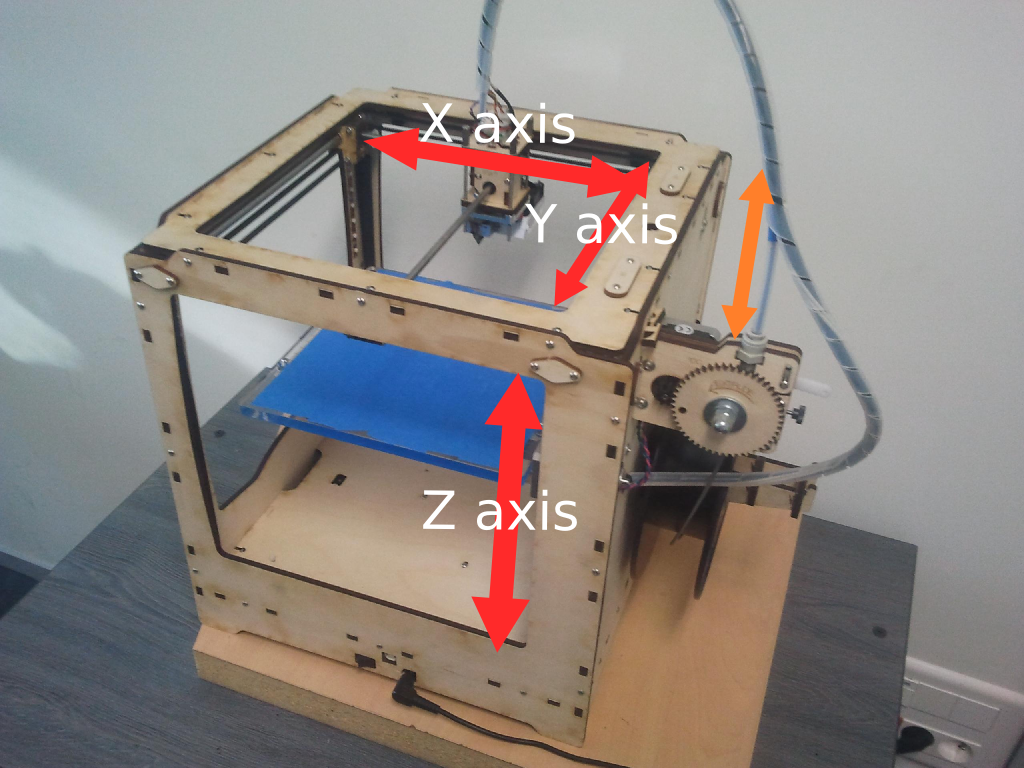
\includegraphics[width=.8\textwidth]{Ultimaker2}	
		\end{center}
    \end{column}

    \end{columns}
    
\end{frame}

\begin{frame}
	\frametitle{In charge: James Packer}

	\begin{block}{The choice of the parameters}
	\begin{itemize}
	\item No perfect set of parameters,
	\item Depends on the printed object,
	\item Basic parameters found:
		\begin{itemize}
		\item temperature: between 210$°C$ and 240$°C$,
		\item layer height: between 0,2 mm  and 0,4 mm,
		\item print speed.
		\end{itemize}
	\end{itemize}	
    \end{block}
    
    \begin{block}{Other options}
    Other tips can improve the efficiency of the printing:	\\
    retraction, infilling, copies, extrusion multiplier...
    \end{block}
\end{frame}

\section{Application and printing limitations}
\begin{frame}
	\frametitle{Limitations}
	
	\begin{block}{Algorithms}
    \begin{itemize}
    \item Mesh correction becomes quite slow for very big meshes,
    \item Mesh correction may be destructive for very damaged meshes,
    \item Automatic supporting planes detection does not work for some objects (like spherical objects),
    \item Gravity center not used $\rightarrow$ might trigger issues.
    \end{itemize}
    \end{block}
    
    \begin{block}{Dual-touch screen}
    The dual-touch only appears to be useful for a few interactions.
    \end{block}
\end{frame}

\begin{frame}
	\frametitle{}

    \begin{center}
    \Large{Thank you for your attention!}
    \end{center}
\end{frame}
	
\end{document}
